\section{Systematic uncertainties}
\label{sec:swave:meas:sys}

There are several distinct sources of systematic uncertainty that are
 considered to affect the measurement of the \kpi S-wave in \BdToKpimm.
The systematic uncertainties affecting the event selection, the corrections to simulation and the model to describe the
\B mass distribution have previously been considered in Section~\ref{sec:kstmm:sys}.
These effects have a possible impact in this analysis and are therefore tested in a similar manner.
There are new sources of systematic uncertainty from the model used for the \mkpi distribution.
These come from both the background and signal models, along with the phase space integration
 assumed over \qsq.
 Each of the sources of systematic uncertainty are discussed below along with the method used to 
 estimate a possible bias.

\subsubsection{The selection}

The possible mis identification of \Kstar and \Kstarb was found in Chapter~\ref{chap:kstmm}  
to be negligible and consequently can be ignored for this measurement.
The amount of \kpi swaps should be negligible due to the cut placed on the \kdllkpi and \pidllkpi combination and is ignored.
The contributions from possible peaking background decays are vetoed to a sufficient degree and similarly ignored.
%however, this cut was varied by so-and-so in order to understand the effect of XXX

\subsubsection{The data-simulation corrections}

The sources of systematic uncertainty that contribute to the corrections applied to the simulation are described in Section~\ref{sec:kstmm:sys}. 
These come from the relative efficiency between the data and the simulation for the tracking, the trigger and the muon identification.
 The smearing of the track IP and the regeneration of the hadron \dll distributions are also possible sources of systematic uncertainty.
The degree of systematic uncertainty contributed by these corrections is evaluated using the same method as described in Section~\ref{sec:kstmm:sys}.

\subsubsection{The acceptance correction}

The factorisation of the efficiency between \psq and \ctk is tested by reducing the range of \ctk.
This removes the contribution from events at high \ctk which may have an erroneous weight applied from the acceptance correction.
The reduction in the range of \ctk changes the model used for the signal since the integral no longer vanishes.
The integral over the angular distribution in terms of \psq, \qsq and \ctk for a symmetric \ctk range is given by
\begin{align}
\int_{-c}^{c} &S(\mkpi,\ctk;\FSi,\ASi,\FL) \,\dctk \nonumber\\
 &= \frac{1}{2} \FSi(\mkpi) (2c) + \FPi(\mkpi) \bigg[ c^3 \FL + \frac{3}{4} ( 1 - \FL ) ( 2c - \frac{2}{3} c^3 ) \bigg]  \, ,
\end{align}
where the term with \ASi vanishes for the symmetric \ctk range. For a \ctk range of less than $-1$ to $1$, 
\FL does not integrate out and a correction is required.

The change in \FS in the \qsq bin from 1 to 6 \gevgevcccc when the \ctk range is changed is shown in Fig.~\ref{fig:fs:ctkrange}.
\begin{figure}[tbp]
\centering
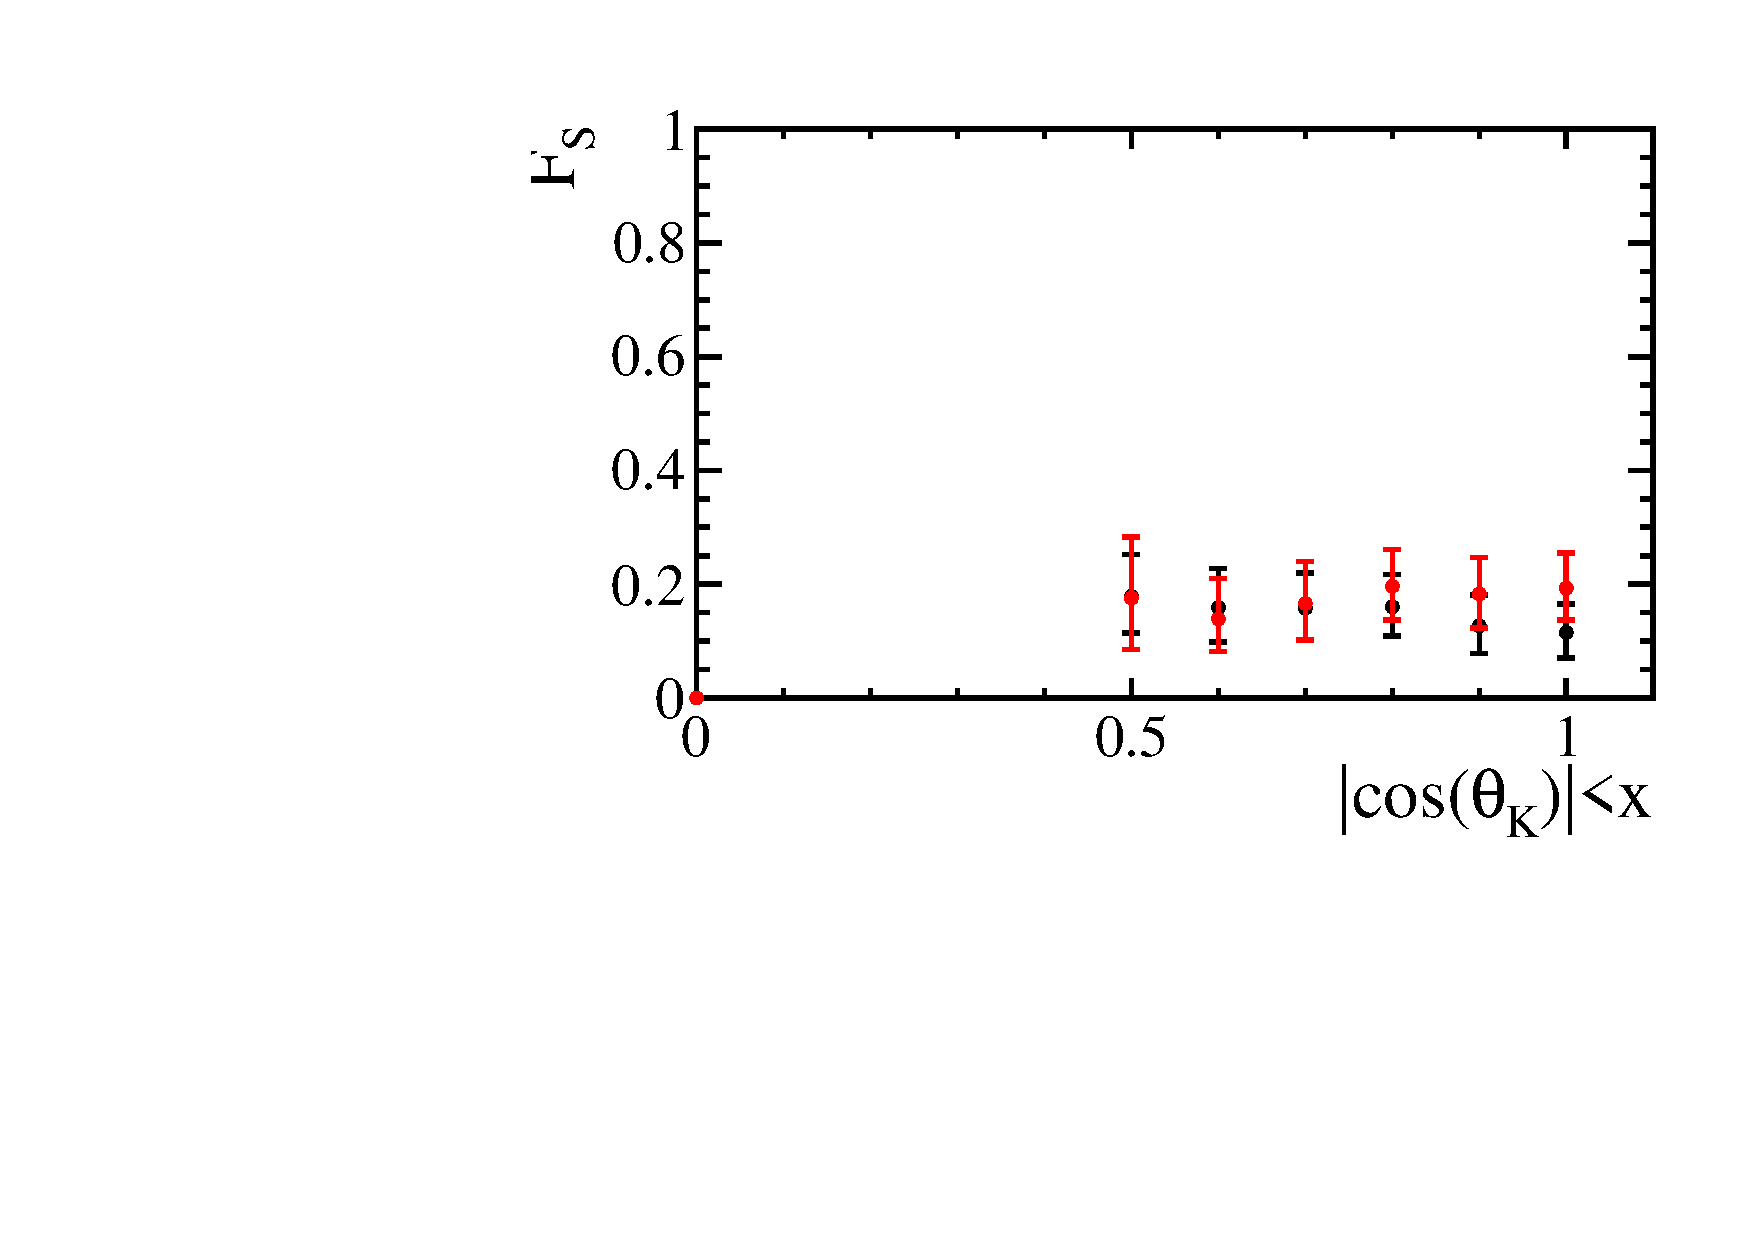
\includegraphics[width=0.48\columnwidth]{chapter7/figs/fiducial_cuts_FS_0.pdf}
\caption[ The change in \FS for different ranges of \ctk.   ]
{The change in \FS for different ranges of \ctk. 
The effect of including events at high \ctk  may contribute to a source of systematic uncertainty.
The change in \FS when only \psq and \qsq is fitted is shown in black and 
the change in \FS when \ctk is included in the angular distribution is shown in \textcolor{red}{red}.
\label{fig:fs:ctkrange} }
\end{figure}
To calculate the correction from the integration, the values of \FL measured in Chapter~\ref{chap:kstmm} are used.
It is possible to see that the results with and without fitting \ctk for different fiducial ranges of \ctk are compatible.
The contribution from this source of systematic uncertainty is chosen to be from the change in \FS when the integration range 
is changed from  $|\ctk|<1$ to $|\ctk|<0.7$.
%Within $|\ctk|<0.7$, the acceptance is flat as seen in Fig.~\ref{fig:fs:ctkrange}.

The integration over \ctk is also checked by fitting the angular distribution in terms of \psq and \ctk.
The acceptance correction from Sec.~\ref{sec:kstmm:ac} is used as an approximation.
The values of \FL obtained from these fits are compatible within statistical errors with the results obtained in Section~\ref{sec:kstmm:res}.
%No systematic uncertainty is assigned from the approximation of the angular distribution by ignoring \ctl and $\phi$.

\subsubsection{The fit model}

There are several possible sources of systematic uncertainty in the choice of model used to describe the \kpimm mass distribution.
The degree to which is \FS  can be affected by the \mB mass distribution comes from the two-stage fit used to obtain the overall fraction of signal in the data for a given region of \qsq.
 In order to test for any bias in the signal shape, the double Crystal Ball function was replaced by a double Gaussian function.
 This will change the tails of the signal distribution and change the quality of the background fit.
In order to test possible uncertainties from the choice of background model, the exponential function was replaced with a second order Chebychev polynomial as the background model.

Following the work in Section~\ref{sec:swave:isobar}, an isobar model consisting of 
a constant non-resonant term, the $\Kstarz(1430)$ and the $\kappa(600)$ was used as an alternative model
the \kpi mass spectrum.

%\subsubsection{uncertainties on the \mkpi model}
%There is a small degree of uncertainty on both the choice of the model for the signal S-wave and the model for the \kpi background.
%[CONCLUSOION].\\
%The use of Equation~\ref{eq:swave:mkpi:background} to model the background \kpi mass spectrum was checked by 
%XXXXXXXXX.
%[CONCLUSOION].\\

The degree to which the approximation of the phase space factor across the \qsq bin effects the final value of \FS is evaluated by using
the \qsq values at both the low and high edge of the \qsq bin in the phase space factor,
\begin{align}
\rho( \mB, \psq,\qsq ) = \left\{ \begin{matrix} \rho( \mB, \psq,\qsq_{max} ) \\\rho( \mB, \psq,\qsq_{min} )   \end{matrix} \right.
\end{align}
This was found to contribute to a minor source of systematic uncertainty.

\subsection{Summary of systematic uncertainties}

The size of possible contributions from sources of systematic uncertainty on the measurement of \FS are given in Table~\ref{tbl:swave:meas:fs:results}.
\begin{landscape}{\scriptsize
\begin{table}[tbp]
\centering
\caption[  Table of possible sources of systematic uncertainty on the measurement of \FS.  ]
{ Table of possible sources of systematic uncertainty on the measurement of \FS. 
Only the bins with a non-zero S-wave contribution are shown.
The bins with no S-wave are unaffected by the possible sources of systematic uncertainty.
 ~\label{tbl:swave:meas:fs:results} }
\begin{tabular}{|c|c|c|c|c|c|c|c|c|}
\hline
\qsq (\gevgevcccc) bin & $0.1<\qsq<2.0$&$2.0<\qsq<4.3$&$4.3<\qsq8.68$&$10.09<\qsq<12.9$&$14.18<\qsq16.0$&$16<\qsq<19$&$1<\qsq<6$\\
Central value & 0.164 & 0.000 & 0.092 & 0.001 & 0.000 & 0.000 & 0.083\\ 
\hline
Stat down & 0.060 & 0.000 & 0.033 & 0.000 & 0.000 & 0.000 & 0.048\\ 
Stat up & 0.069 & 0.135 & 0.039 & 0.044 & 0.007 & 0.002 & 0.057\\ 
\hline
Sys down & 0.013 & 0.000 & 0.046 & 0.000 & 0.000 & 0.000 & 0.050\\ 
Sys up & 0.011 & 0.001 & 0.021 & 0.000 & 0.000 & 0.000 & 0.018\\ 
\hline
Bkg order 1 & 0.000 & 0.000 & 0.000 & 0.000 & 0.000 & 0.000 & -0.026\\ 
Bkg order 3 & 0.000 & 0.000 & 0.000 & 0.000 & 0.000 & 0.000 & 0.000\\ 
PID down  & 0.000 & 0.000 & 0.000 & 0.000 & 0.000 & 0.000 & 0.000\\ 
PID up & 0.000 & 0.000 & 0.000 & 0.000 & 0.000 & 0.000 & 0.000\\ 
fit the \B mass & 0.000 & 0.000 & -0.001 & 0.000 & 0.000 & 0.000 & 0.003\\ 
isobar model & 0.000 & 0.000 & 0.000 & 0.000 & 0.000 & 0.000 & 0.000\\ 
Muon ID down & 0.000 & 0.000 & -0.029 & 0.000 & 0.000 & 0.000 & 0.000\\ 
Muon ID up & 0.000 & 0.000 & 0.000 & 0.000 & 0.000 & 0.000 & 0.000\\ 
IP smearing & 0.000 & 0.000 & -0.029 & 0.000 & 0.000 & 0.000 & 0.000\\ 
\qsq efficiency  down & 0.000 & 0.000 & 0.000 & 0.000 & 0.000 & 0.000 & 0.000\\ 
\qsq efficiency up & 0.000 & 0.000 & 0.000 & 0.000 & 0.000 & 0.000 & 0.000\\ 
\ctk limit & -0.008 & 0.001 & 0.001 & 0.000 & 0.000 & 0.000 & -0.029\\ 
\qsq high edge & -0.010 & 0.000 & -0.020 & 0.000 & 0.000 & 0.000 & -0.018\\ 
\qsq low edge & 0.011 & 0.000 & 0.021 & 0.000 & 0.000 & 0.000 & 0.018\\ 
Tracking Down & 0.000 & 0.000 & 0.000 & 0.000 & 0.000 & 0.000 & 0.000\\ 
Tracking Up & 0.000 & 0.000 & 0.000 & 0.000 & 0.000 & 0.000 & 0.000\\ 
Trigger Down & 0.000 & 0.000 & 0.000 & 0.000 & 0.000 & 0.000 & -0.026\\ 
Trigger Up & 0.000 & 0.000 & 0.000 & 0.000 & 0.000 & 0.000 & 0.000\\ 
\hline
\end{tabular}
\end{table}}
\end{landscape}
The dominant sources of systematic uncertainty come from the use of the crystal ball function to fit the \kpimm invariant mass
and from the mis-modelling of the \qsq and \psq efficiency.




